One constraint in this project is to build two different classifiers to compare their efficiency. So we choose to build one classifier based on the style of writing (punctuation, number of words per sentence ...) and one based on the content of the article (adjectives, common words...).

Here is a graphical recap of how the project is structured.
\begin{figure}[h]
	\centering
		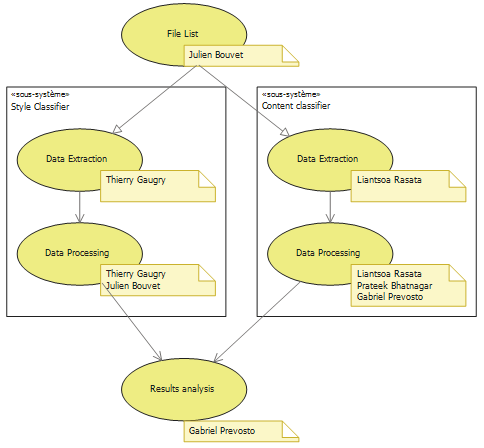
\includegraphics{Images/organization.png}
	\caption{Organization}
	\label{fig:organization}
\end{figure}
